\documentclass{UoNMCHA}
\usepackage[authoryear]{natbib}
\usepackage{array,booktabs} % For nice tables
\usepackage{amsmath,amsfonts,amssymb} % For nice maths
\usepackage{color}
\usepackage{enumerate}
\usepackage{listings}
\usepackage{subfig}
\usepackage{hyperref}
\usepackage[parfill]{parskip}   % For replacing paragraph indenting with a newline instead
\usepackage{textcomp}
\usepackage{caption}
\usepackage{floatrow}
\usepackage{tabularht}
\usepackage[table,xcdraw]{xcolor}
\usepackage{hyperref}
\usepackage{blindtext}
\usepackage[bottom]{footmisc}


% Number equations per section
\numberwithin{equation}{section}

\usepackage{float}
\floatstyle{plaintop}
\restylefloat{table}

\hypersetup{
%    bookmarks=true,         % show bookmarks bar?
%    unicode=false,          % non-Latin characters in AcrobatÕs bookmarks
%    pdftoolbar=true,        % show AcrobatÕs toolbar?
%    pdfmenubar=true,        % show AcrobatÕs menu?
%    pdffitwindow=false,     % window fit to page when opened
%    pdfstartview={FitH},    % fits the width of the page to the window
%    pdftitle={My title},    % title
%    pdfauthor={Author},     % author
%    pdfsubject={Subject},   % subject of the document
%    pdfcreator={Creator},   % creator of the document
%    pdfproducer={Producer}, % producer of the document
%    pdfkeywords={keyword1} {key2} {key3}, % list of keywords
%    pdfnewwindow=true,      % links in new window
    colorlinks=true,       % false: boxed links; true: colored links
    linkcolor=blue,          % color of internal links
    citecolor=blue,        % color of links to bibliography
%    filecolor=magenta,      % color of file links
    urlcolor=blue           % color of external links
}

\definecolor{MATLABKeyword}{rgb}{0,0,1}
\definecolor{MATLABComment}{rgb}{0.1328125,0.54296875,0.1328125}
\definecolor{MATLABString}{rgb}{0.625,0.125,0.9375}

\lstset{language=Matlab,
    basicstyle=\small\ttfamily,
    keywordstyle=\color{MATLABKeyword},
    %identifierstyle=,
    commentstyle=\color{MATLABComment},
    stringstyle=\color{MATLABString},
    numberstyle=\tiny,
    %numbers=left,
    basewidth=0.5em}

\firstpage{1}    % Set page number for first page
\UoNMCHAreportNo{MCHA3000 Report} %Report number
\UoNMCHAyear{2018}   % Year
\shorttitle{Self-balancing Inverted Pendulum Robot} %For odd pages
%%%%%%%%%%%%%%%%%%%%%%%%%%%%%%%%%%%%%%%%%%%%%%%%%%%%
\begin{document}
\title{Type II Inverted Pendulum Robot \\ \ \\
{\small Major Project for MCHA 3000  \\November 2018}}
\author[UoNMCHA]{Muhammad Hasham Khan}
\address[UoNMCHA]{
Student of Mechatronics Engineering,\\
The University of Newcastle, Callaghan, NSW 2308, AUSTRALIA \\
Student Number: 3256011 \\
E-mail: \href{mailto:c3256011@uon.edu.au}{\textsf{c3256011@uon.edu.au}}}
%%%%%%%%%%%%%%%%%%%%%%%%%%%%%%%%%%%
\maketitle
\onecolumn

\vspace{-5mm}
\section*{Abstract}
\vspace{-3mm}
    
    This report encompasses the design, construction and commissioning of an inverted pendulum robot, a major project undertaken by Bachelor of Mechtronics Engineering students in their third year of study at the University of Newcastle. The project challenges students to control a non-linear system using system analysis, control theory, circuit design, material analysis, dynamic modeling and embedded system programming, a process involves addressing and optimizing conflicting design objectives within provided constraints. \\
    
    The Report establishes the Project and its constraints, explores the mathematical modeling behind the chosen system and the subsequent hardware design and selection. It then explores the techniques used to identify system parameters and explores how the simulation model was constructed. The system is then tested and commissioned and subsequently evaluated. \\
     
    The design was ultimately only partially successful with limited stability and velocity tracking ,  reasons for which include poor system identification and lack of proper state estimation. 
    

\newpage
\tableofcontents
\newpage
%%%%%%%%%%%%%%%%%%%%%%%%%%%%%%%
\section{Introduction}
%To organise your introduction section you can use the following structure:
%\begin{itemize}
%    \item \textbf{Position}: Show there is a problem and that it is important to solve it.
%   
Third year Mechatronics Engineering students at the University of Newcastle are eligible to enrol in Mechatronics System Design I (MCHA 3000), a  major project oriented course focusing on controlling an unstable, non-linear system. This course aims to challenge a students ability to draw upon the fundamental concepts of system analysis, control theory, circuit design, material analysis, dynamic modeling and embedded system programming as well as demonstrate proficiency in utilizing design tools such as Creo Paramatetric\textsuperscript{\texttrademark}, Eagle\textsuperscript{\texttrademark} and Matlab\textsuperscript{\texttrademark}. It also tests their ability to address conflicting design objectives, such as maximizing material strength while minimizing weight, and optimize a design subject to constraints, such as cost and time.\\ 

Thus, the project for 2018 was chosen and students were tasked with stabilizing an inverted pendulum robot, an inherently unstable and non-linear system, and control it's velocity along the ground. They were presented with two options; An inverted pendulum on a cart (Type I), as shown in Figure \ref{TypeIrobot}, or a more challenging free-standing robot (Type II), as shown in Figure \ref{TypeIIrobot}.



\begin{figure}[!h]
	\begin{floatrow}
		\ffigbox{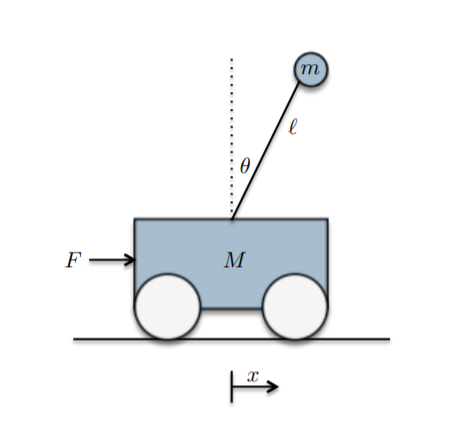
\includegraphics[scale = 0.8]{figs/TypeIrobot}}{\caption{Inverted pendulum on a cart}\label{TypeIrobot}}
		\ffigbox{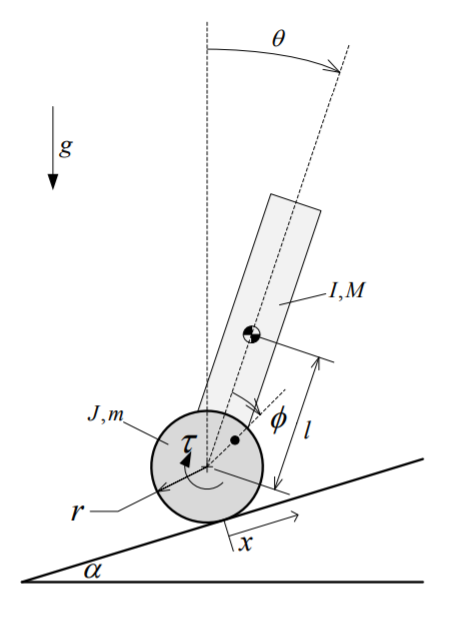
\includegraphics[scale = 0.8]{figs/TypeIIrobot}}{\caption{Free-standing robot}\label{TypeIIrobot}}
	\end{floatrow}
\end{figure}
    
\newpage
Students were also presented with a series of design constraints for the project:

\begin{itemize}
    \item All onboard computation performed on supplied STM32F411 Nucleo-64 clocked at 100MHz
    \item The robot must not be mechanically self-stabilising in an unpowered state
    \item The pendulum joint (for Type I) must not be directly driven by an actuator mounted between
    the chassis and the pendulum
    \item Any angle sensing device attached to the pendulum joint (for Type I) must not introduce excessive mechanical friction
    \item The robot center of gravity (including the pendulum for Type I) must be above all axes of wheels that are in contact with the ground during operation.

\end{itemize}

The final project was assessed based on 5 criteria: Hardware design, Software coding, System identification, Simulation model and Control design as well as a practical demonstration. \\

 This report will cover the design and commisioning of a type II robot, which was selected due to its challenging nature and interesting dynamics. \\ 
 Section \ref{Math} explores the mathematical model used to simulate the system and the Lagrangian equations used in its derivation. Section \ref{Hardware} explores the hardware design selection and construction, Section \ref{SysID} analyses the chosen hardware using system identification, Section \ref{Simulation} simulates the chosen model paramaters and Section \ref{Testing} covers it's testing. Finally, Section \ref{Conclusion} explores the success of the robot and reflects on the project as a whole.


\newpage
\section{Mathematical Model}\label{Math}

In order to properly design the robot, we must first derive a mathematical model to use as a basis for all subsequent design and analysis. This process involves creating a Free-Body diagram and then computing the systems Euler-Lagrangian equations.
\subsection{Free-Body Diagram}

Figure \ref{TypeIIrobot} was already provided as a Free-Body diagram of the system and demonstrates the models dynamics.

\subsection{Euler-Lagrangian Equations}

The equations of motion for this system are derived by computing the Lagrangian, $\mathcal{L}(q,\dot{q}) = \mathcal{T\textsuperscript{*}}(q,\dot{q}) - \mathcal{V}(q) = \frac{1}{2}\dot{q}\textsuperscript{T}M(q)\dot{q} - \mathcal{V}(q)$ ,  for the generalized coordinates $q = [\phi, \theta]\textsuperscript{T}$. They are then substituted into the Euler-Lagrange equations to obtain the following model:

\begin{equation}\label{Lagrangian}
\begin{split}
\frac{d}{dt}(\frac{\partial\mathcal{L}}{\partial\dot{q}}) - \frac{\partial\mathcal{L}}{\partial{q}} = \tau \\
\frac{d}{dt}(M(q)\dot{q}) - \frac{\partial\mathcal{T\textsuperscript{*}}}{\partial{q}}  + \frac{\partial\mathcal{V}}{\partial{q}} = \tau \\
M(q)\ddot{q} + \dot{M}(q)\dot{q} - \frac{\partial\mathcal{T\textsuperscript{*}}}{\partial{q}}  + \frac{\partial\mathcal{V}}{\partial{q}} = \tau \\ 
\end{split}
\end{equation}

%\begin{equation}\label{Lagrangian_derived}
%\begin{split}
%	\mathcal{L}(\dot{\phi},\phi,\dot{\theta},\theta) ={} & \frac{1}{2}(J + (M + m)r\textsuperscript{2})(\dot{\phi} + \dot{\theta})\textsuperscript{2}
%	+ Mlr(\dot{\phi} + \dot{\theta})\dot{\theta}cos(\theta + \alpha) \\  
%	&\quad + \frac{1}{2}(I + Ml\textsuperscript{2})\dot{\theta}\textsuperscript{2} - (M + m)gr(\phi + \theta)sin(\alpha) - Mglcos(\theta)
%	\end{split}
%\end{equation}


Factorizing the kinetic co-energy into quadratic form,
 $\mathbf{\mathcal{T\textsuperscript{*}}}= \frac{1}{2}\dot{q}^{\tau}M(q)\dot{q}$ , taking 
  $\mathbf{C(q,\dot{q})\dot{q}} = \dot{M}(q)\dot{q}-\frac{\delta\tau^*}{\delta q}$
   and $\mathbf{g(q)}=\frac{\delta v}{\delta q}$, and finding ,$\mathbf{\tau}$, to maintain a stationary balancing angle, yields:

\begin{equation}
\mathbf{\mathcal{T\textsuperscript{*}}} = \frac{1}{2}\dot{q}^{T}
\begin{bmatrix}
J+(M+m)r^2 & J+(M+m)r^2+Mlrcos(\theta+\alpha) \\
J+(M+m)r^2+Mlrcos(\theta+\alpha) & J+(M+m)r^2+2Mlrcos(\theta+\alpha)+I+Ml^2  \\
\end{bmatrix}\dot{q}
\end{equation}

\begin{equation}
\mathbf{C(q,\dot{q})\dot{q}} = 
\begin{bmatrix}
-Mlrsin(\theta+\alpha)\dot\theta^2\\
-Mlrsin(\theta+\alpha)\dot\theta^2\\
\end{bmatrix}
\end{equation}
\begin{equation}
\mathbf{g(q)} = 
\begin{bmatrix}
(M+mgrsin(\alpha))\\
(M+mgrsin(\alpha))-Mglsin(\theta)\\
\end{bmatrix}
\end{equation}

which can be substituted into \ref{Lagrangian} to provide non-linear model of the system.
In order to design a linear controller, a linear state space model is required. Therefore, linearize the Lagrangian (\ref{Lagrangian}) using a Taylor series expansion around the origin at $ \theta_0=\dot{\theta_0}=\ddot{\theta_0}=\ddot{\phi_0}=0$ gives:

\begin{equation}\label{2.5}
\mathbf{M\ddot{q} + D\dot{q} + Kq = \tau}  
\end{equation}
where: 
\begin{equation}
\mathbf{M} = 
\begin{bmatrix}
(J+(M+m)r^2) & (J+(M+m)r^2)+Mlr\\
(J+(M+m)r^2)+Mlr & (J+(M+m)r^2)+2Mlr+(I+Ml^2)  \\
\end{bmatrix}
\end{equation}

\begin{equation}
\mathbf{D} = 
\begin{bmatrix}
0 & 0\\
0 & 0 \\
\end{bmatrix}
\end{equation}

\begin{equation}
\mathbf{K} = 
\begin{bmatrix}
0 & 0\\
0 & -Mgl \\
\end{bmatrix}
\end{equation}

Rearranging \ref{2.5} to give $\ddot{q} = M\textsuperscript{-1}(-D\dot{q} - Kq + \tau)$ and taking $v=\dot{q}$ gives (in state space form):

\begin{equation}
\begin{bmatrix}
\dot{v} \\
\dot{q} \\
\end{bmatrix} = 
\begin{bmatrix}
-M\textsuperscript{-1}D & -M\textsuperscript{-1}K\\
I & 0 \\
\end{bmatrix}
\begin{bmatrix}
v\\
q\\
\end{bmatrix}
+
\begin{bmatrix}
M\textsuperscript{-1}b\\
0\\
\end{bmatrix}
\end{equation}

where $b = 0$. 
This model can now be used to derive a Controllable and Observable model of the system.

\newpage
\section{Hardware Design}\label{Hardware}

The hardware design of the Type II robot incorporates the design and construction of the chassis,suitable actuator selection and appropriate power electronics.

\subsection{Material Selection}

There are a variety of materials, such as aluminium, carbon fiber and acrylic, which were considered for their properties and Table \ref{material} shows how they were evaluated

% Please add the following required packages to your document preamble:
% \usepackage{graphicx}
% \usepackage[table,xcdraw]{xcolor}
% If you use beamer only pass "xcolor=table" option, i.e. \documentclass[xcolor=table]{beamer}
\begin{table}[!h]
	\caption{Weighted performance criteria for material selection}
	\label{material}
	\resizebox{\textwidth}{!}{%
		\begin{tabular}{|c|c|c|c|c|c|c|}
			\hline
			\textbf{Criteria}             & \textbf{Weighting} & \textbf{Aluminum} & \textbf{Acrylic} & \textbf{Plastic (3D print)}  & \textbf{Carbon fiber} & \textbf{Steel} \\ \hline
			\textbf{Weight}               & 10                 & 75                & 75               & 85   & 85                    & 30             \\ \hline
			\textbf{Cost}                 & 40                 & 60                & 60               & 90   & 10                    & 50             \\ \hline
			\textbf{Strength}             & 20                 & 75                & 50               &60   & 90                    & 75             \\ \hline
			\textbf{Ease of Construction} & 30                 & 60                & 50               &90   & 50                    & 50             \\ \hline
			\textbf{Weighted Score}       & 100                & 6450              & 5650             & \cellcolor[HTML]{32CB00}8350 & 4550                  & 5300           \\ \hline
		\end{tabular}%
	}
\end{table}

Thus, a 3D printed plastic chassis was ultimately chosen as it was light, cheap, easy to manufacture and had the added benefit of being an electric insulator, preventing short-circuits.\\

\subsection{Actuator Selection}

The available choices for actuators were narrowed down to a choice between stepper motors and brushed DC motors. Stepper motors have the advantage of having high holding torque and requiring basic system identification. Conversely, DC motors have higher RPM, greater efficiency and less operational vibration at the cost of requiring extensive system identification. \\

Ultimately, DC motors were chosen and the \textit{Pololu 19:1 Metal Gearmotor 37Dx68L mm with 64 CPR Encoder}\footnote{Details found in Appendix \ref{BOM}} was selected as it had a high encoder resolution, suitable torque output and high RPM. \\ 
These motors required powerful motor drivers, which is why the \textit{VNH5019 Motor Driver Carrier}\footnotemark[\value{footnote}] was selected

\subsection{Sensors and Power Electronics}

The mathematic model derived in Section \ref{Math} had states ,$\dot{\phi}, \phi,  \dot{\theta}$ and $\theta$. Of these states, $\phi$ could be measured using an encoder(bundled with the actuator) while $\dot{\theta}$ and $\theta$ could be measured using an \textit{MPU-6050}\footnotemark[\value{footnote}]; a cheap, light and robust Inertial Measurement Unit(IMU). \\

Additionally, a few now-essential but useful components were selected; A  \textit{HC-05 bluetooth module}\footnotemark[\value{footnote}] was chosen for wireless communication, Current sensors, \textit{ACS711EX}\footnotemark[\value{footnote}] , were  purchased to provide additional voltage regulation and A \textit{LCD}\footnotemark[\value{footnote}] was selected to display useful information such as current Chassis angle. 

\subsection{Battery}

A large battery, the \textit{Turnigy 5000mAh 3S 30C-40C Lipo}\footnotemark[\value{footnote}], was chosen to maximize endurance and raise the center of gravity of the chassis (for reasons covered in subsection \ref{design}). This battery also had a high discharge rate, which would be needed for scenarios requiring high-torque from the motors.

\subsection{Design and Construction}\label{design}

While designing the Chassis and PCB, there were many design trade-offs to consider.

As found in Assignment 1, increasing the length of the pendulum \textit{l} by raising the center of gravity of the chassis and decreasing the overall mass, would minimise the bode sensity integral and thus the \href{https://tinyurl.com/y7e8eue4}{waterbed effect}. This would improve the control envelope and  thus the battery was placed as high as possible and the overall chassis weight was minimized by only designing a rigid frame. This decision had the added benefit of providing cooling for the power electronics and minimized the effects of air resistance, reducing the control force required to balance. The bottom of the chassis was also shaped to fit the motors to minimize vibrations and maximize clearance. \\

The Creo model of the robot is shown in Figure \ref{Creomodel} and the end product in Figure \ref{robotphoto}

\begin{figure}[!h]
	\begin{floatrow}
		\ffigbox{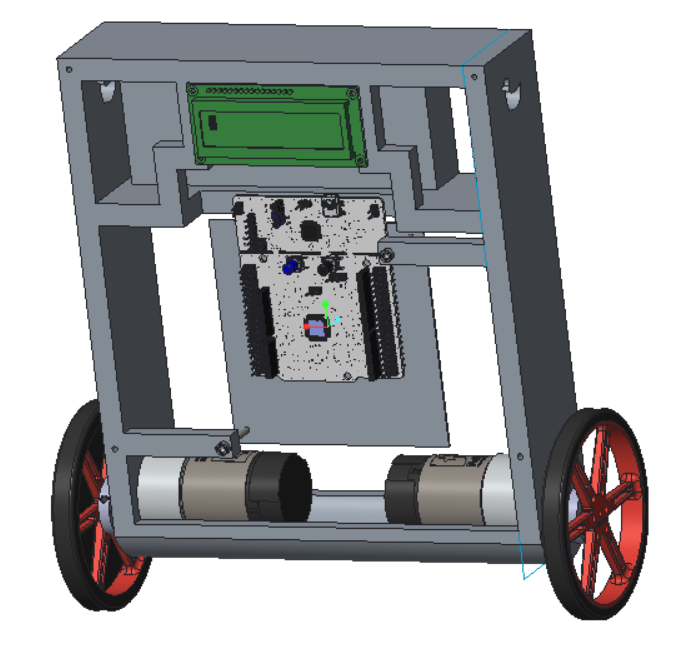
\includegraphics[scale = 0.5]{figs/Creomodel}}{\caption{Creo Model of the Robot}\label{Creomodel}}
		\ffigbox{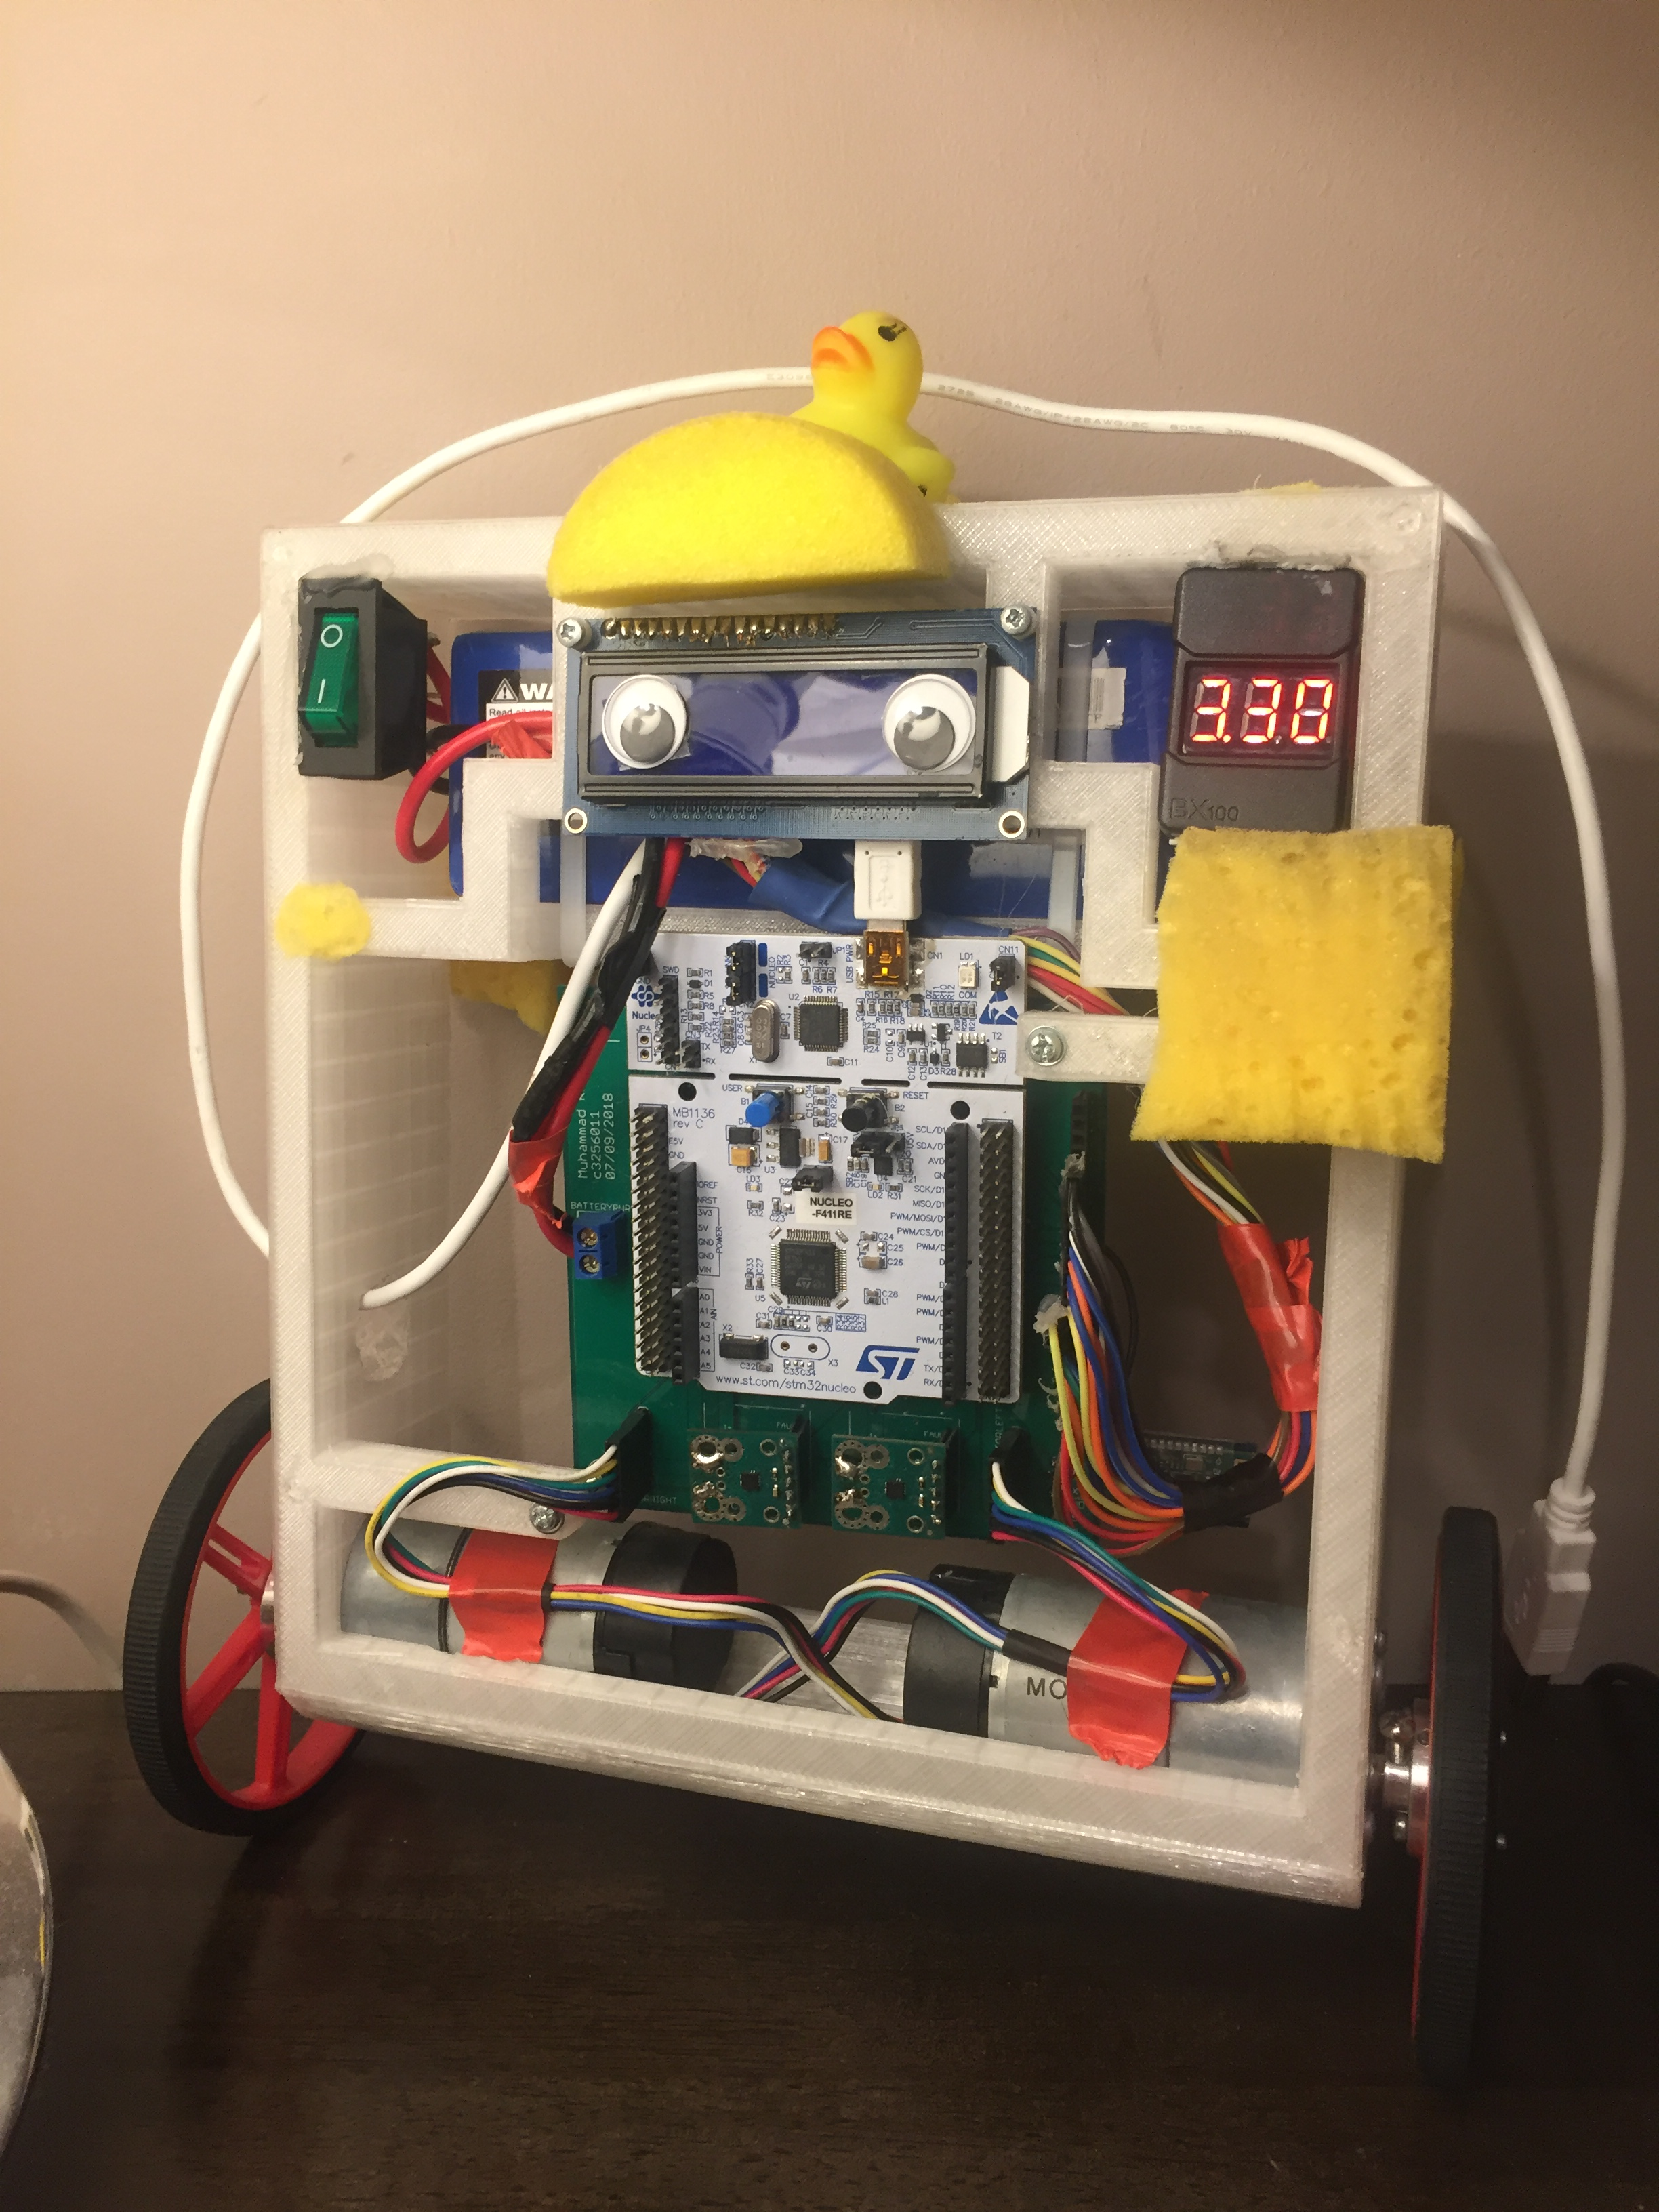
\includegraphics[scale = 0.06]{figs/robotphoto}}{\caption{Constructed and Assembled Robot}\label{robotphoto}}
	\end{floatrow}
\end{figure}


\newpage
\section{System Identification}\label{SysID}

In order to create an accurate Simulation model, we must have accurate system parameters. Some of these can be measured, such as weight and radius, while others can only be found through system identification, such as the inertia of the chassis or the resistance of the motor. \\
 Data sheets can be used to provide expected values, although proper system identification  allows for more accurate values to be obtained and thus more precise control.\\
Thus, in order to improve the system model, system identification was performed on the chassis, motor.

\subsection{Chassis System Identification}

The chassis of the Type II robot is modeled as an inverted pendulum, whose equation is given by:

\begin{equation}\label{Invpend}
	ml\textsuperscript{2}\dot{\dot{\theta}} + (c+b)\dot{\theta} + mglsin(\theta) = 0
\end{equation}

where \textit{l, c, b} and $I= ml\textsuperscript{2}$ are unknown parameters. \\

These parameters were estimated by performing a pendulum swing test. This involved attaching the chassis via the motor shaft to an encoder, allowing it to swing freely, and measuring the change in its angle over time.\\
A Simulink model was then used, based on equation \ref{Invpend}, to obtain the theoretical change in its angle over time. The two sets of experimental and simulated data were then plotted together and curve fitting was used to ensure the modeled system matched the experimental one, as shown in Figure \ref{training}.

\begin{figure}[!h]
	\begin{center}
		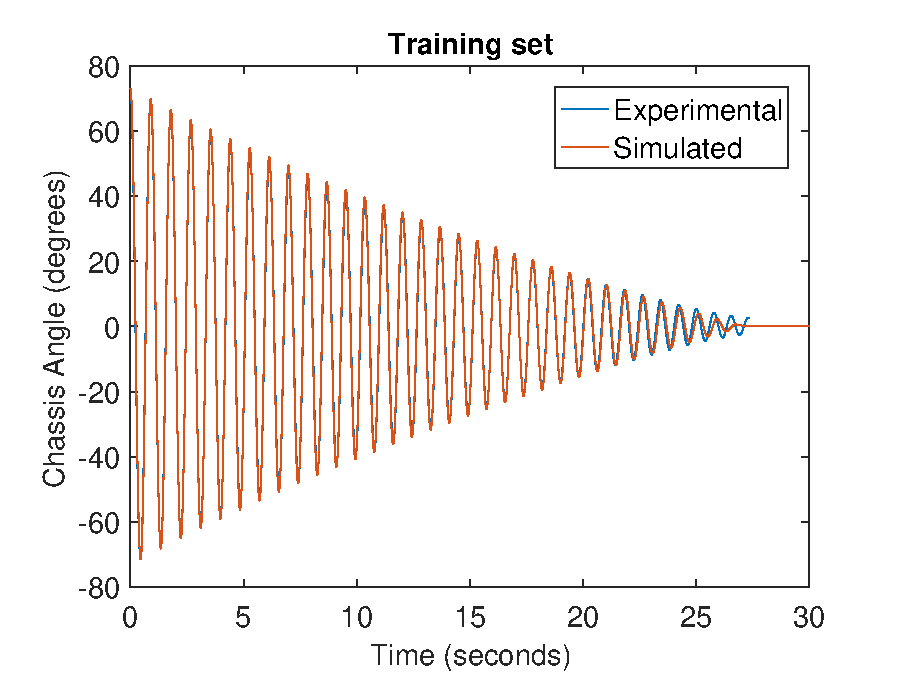
\includegraphics[width=.6\linewidth]{figs/trainingset}
		\caption{Fitting a Simulated swing to an Experimental swing}
		\label{training}
	\end{center}
\end{figure}

Another experimental swing was then performed in order to validate the estimated system parameters and exhibit how well they model the actual chassis. The results of the validation test are shown in Figure \ref{validation}.

\begin{figure}[!h]
	\begin{center}
		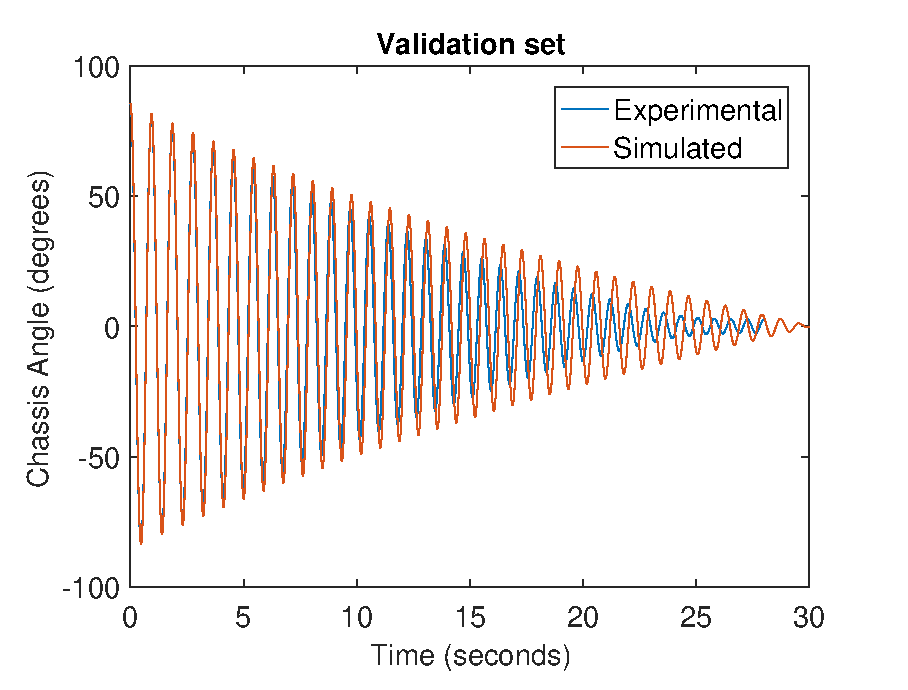
\includegraphics[width=.6\linewidth]{figs/validationset}
		\caption{Validation of the System Parameters}
		\label{validation}
	\end{center}
\end{figure}

Although the frequency of the validation set matches the training set, the simulation seems to be under-damped and not settle as quickly as the actual chassis. This occurs due to experimental error, as lubricant was used during the testing set to ensure minimal friction damping while it was accidentally neglected in the validation set. Thus, the under-damping is accounted for and the model accurately matches the actual chassis, although further validation testing would be recommended.


\subsection{Motor System Identification}

In order to find the internal parameters of the gearbox motor, Kirchoff's voltage law was applied to the DC motor model provided in Assignment 1: 

\begin{equation}\label{kirchoff}
	U - Ri - L\frac{di}{dt} - K\omega\textsubscript{i} = 0
\end{equation}

Assignment 1 also gave the equation:

\begin{equation}\label{taum}
(K\eta)IN - (\tau\textsubscript{m}\eta)N = \tau\textsubscript{L}
\end{equation}

and the unknown motor parameters were thus :\textit{R, K, $\eta$} and \textit{$\tau\textsubscript{m}$}. These values could be obtained via a motor system identification experiment.\\\\
The experiment was performed by coupling the motor shaft to a flywheel of known radius, attached to which via a chord is a known mass. The motor was run at 12V at 100\% duty cycle and its angular displacement ($\phi$) over time measured using an encoder and its current consumption measured using a current sensor. This process was repeated while varying the mass in order to get a large sample set.\\

This data was then used to find the average current(I) and angular velocity($\omega$) at different torque loads for each motor, as shown in Figures \ref{current} and \ref{dphi} respectively.

\begin{figure}[!h]
	\begin{floatrow}
		\ffigbox{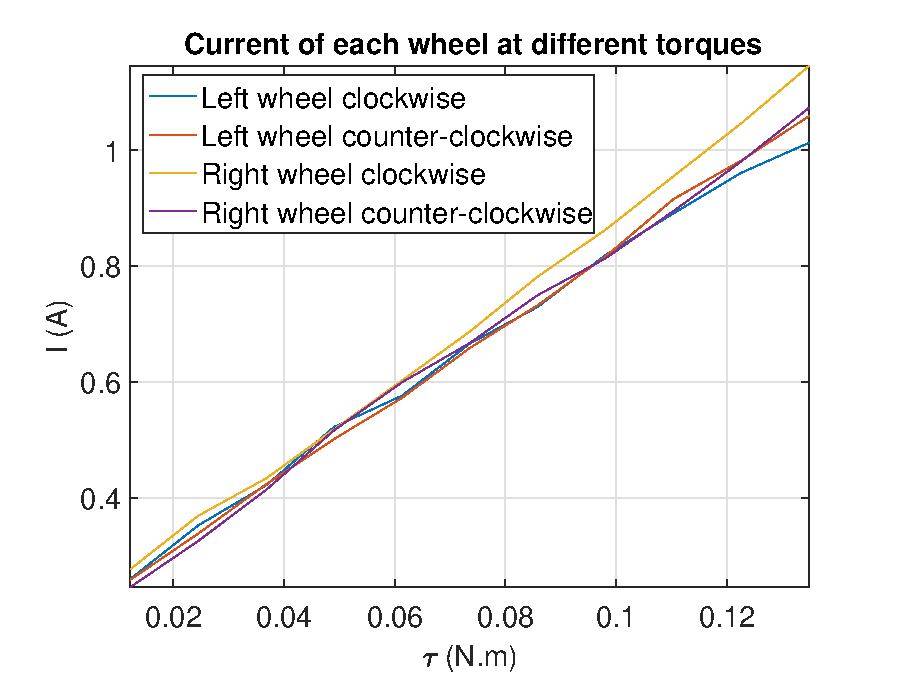
\includegraphics[scale = 0.6]{figs/current}}{\caption{Motor Current at different $\tau$}\label{current}}
		\ffigbox{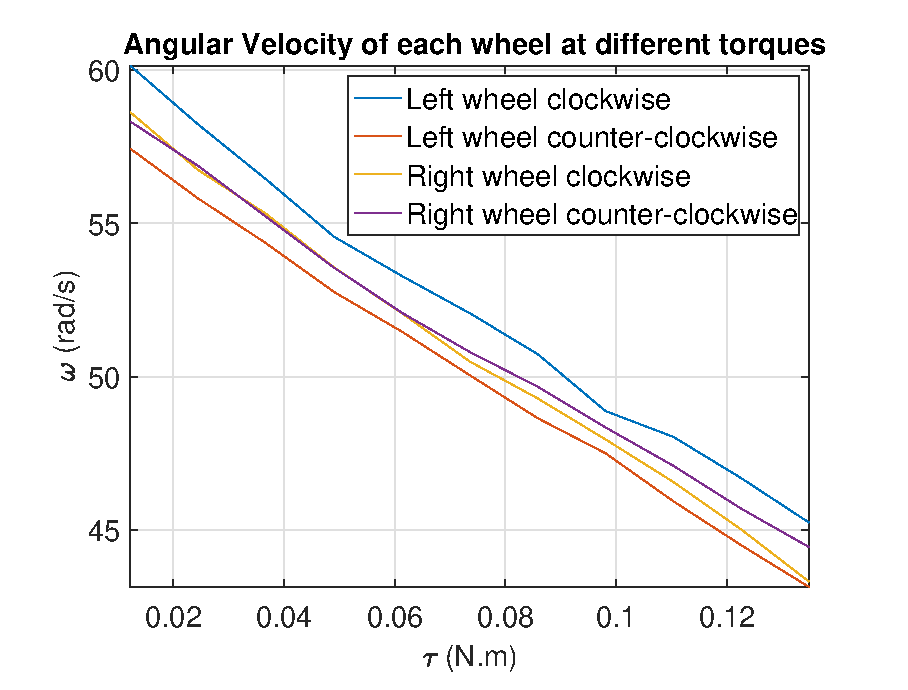
\includegraphics[scale = 0.6]{figs/dphi}}{\caption{Motor $\omega$ at different $\tau$}\label{dphi}}
	\end{floatrow}
\end{figure}

Least squares was then applied using these values and equations \ref{kirchoff} (where $\frac{di}{dt}= 0$ at steady state) and \ref{taum} to find the motor parameters for each motor, as shown in Table \ref{motorsysid}

\begin{table}[!h]
	\caption{My caption}
	\label{motorsysid}
	\resizebox{\textwidth}{!}{%
		\begin{tabular}{lllllll}
			\cline{1-5}
			\multicolumn{1}{|l|}{\textbf{Parameter}} & \multicolumn{1}{l|}{\textbf{Left clockwise}} & \multicolumn{1}{l|}{\textbf{Left counterclockwise}} & \multicolumn{1}{l|}{\textbf{Right clockwise}} & \multicolumn{1}{l|}{\textbf{Right counterclockwise}} &  &  \\ \cline{1-5}
			\multicolumn{1}{|l|}{Resistance \textit{R} ($\Omega$)}  & \multicolumn{1}{l|}{3.545600379}             & \multicolumn{1}{l|}{3.411528473}                    & \multicolumn{1}{l|}{3.290337899}              & \multicolumn{1}{l|}{3.257610086}                     &  &  \\ \cline{1-5}
			\multicolumn{1}{|l|}{Motor constant \textit{K} ()}  & \multicolumn{1}{l|}{0.009883413}             & \multicolumn{1}{l|}{0.010368676}                    & \multicolumn{1}{l|}{0.010184167}              & \multicolumn{1}{l|}{0.010274251}                     &  &  \\ \cline{1-5}
			\multicolumn{1}{|l|}{efficiency \textit{$\eta$} (\%)}         & \multicolumn{1}{l|}{0.868793132}             & \multicolumn{1}{l|}{0.783533109}                    & \multicolumn{1}{l|}{0.787743734}              & \multicolumn{1}{l|}{0.780836803}                     &  &  \\ \cline{1-5}
			\multicolumn{1}{|l|}{taum \textit{$\tau\textsubscript{m}$}(N.m)}         & \multicolumn{1}{l|}{-0.002716981}            & \multicolumn{1}{l|}{-0.002669111}                   & \multicolumn{1}{l|}{-0.00258998}              & \multicolumn{1}{l|}{-0.002612889}                    &  &  \\ \cline{1-5}
			&                                              &                                                     &                                               &                                                      &  & 
		\end{tabular}%
	}
\end{table}

\subsection{Motor Inertia System Identification}

An attempt was made to find, via experiment and simulation, the inertia of the motor (J), which encompassed the linked inertia of the wheels, the wheel hubs and the gears of the motor and could thus not be individually derived.\\

From our motor system identification experiment, we know the angular velocity ($\omega$) of our motor shaft over time. There is an initial transient state which is then followed by a steady state as the motor reaches speed. The two parameters responsible for the transient behaviour are inductance of the motor (L) and Inertia of the motor (J). If we assume the inductance is negligible compared to the inertia, we can then perform a simulation of the experiment using our model of the gearbox and use curve fitting to find a value for J. The results are found in Appendix \ref{JsysID} and the Inertia was estimated to be $J =  0.001 kg.m\textsuperscript{2}$


\newpage
\section{Simulation Model and Controller Design}\label{Simulation}

	
Matlab was used to simulate the Type II robot, using the model derived in Section \ref{Math}, and design an appropriate controller.

\subsection{Plant Model}

There are two models we need to consider when designing an output feedback controller for the system;The controllable model and the observable model.

The controller aims to regulate the ground velocity of the type II robot, given by $y\textsubscript{ctrl} = r(\dot{phi} + \dot{theta})$. Since one of the design criteria for the robot is to achieve stability at a constant ground velocity, the state $\phi$ would grow unbounded with time. To overcome this, $phi$ was removed from the state vector.\\
The resultant controllable system was then regulated using an LQR controller, as shown in \citep{Franklin}

The observable models aim is to estimate the states of the system based on data provided by the sensors and knowledge of the plant model. An additional state was required to due to bias in the gyroscope and the resultant system was then observed using a kalman filter, as shown in \citep{Franklin}

\subsection{Motor Model and Control Allocation}

A motor plant model, found in Figure \ref{Motormodel}, was developed in Assignment 1 and used to simulate the dynamics of each motor.\\

\begin{figure}[!h]
	\begin{center}
		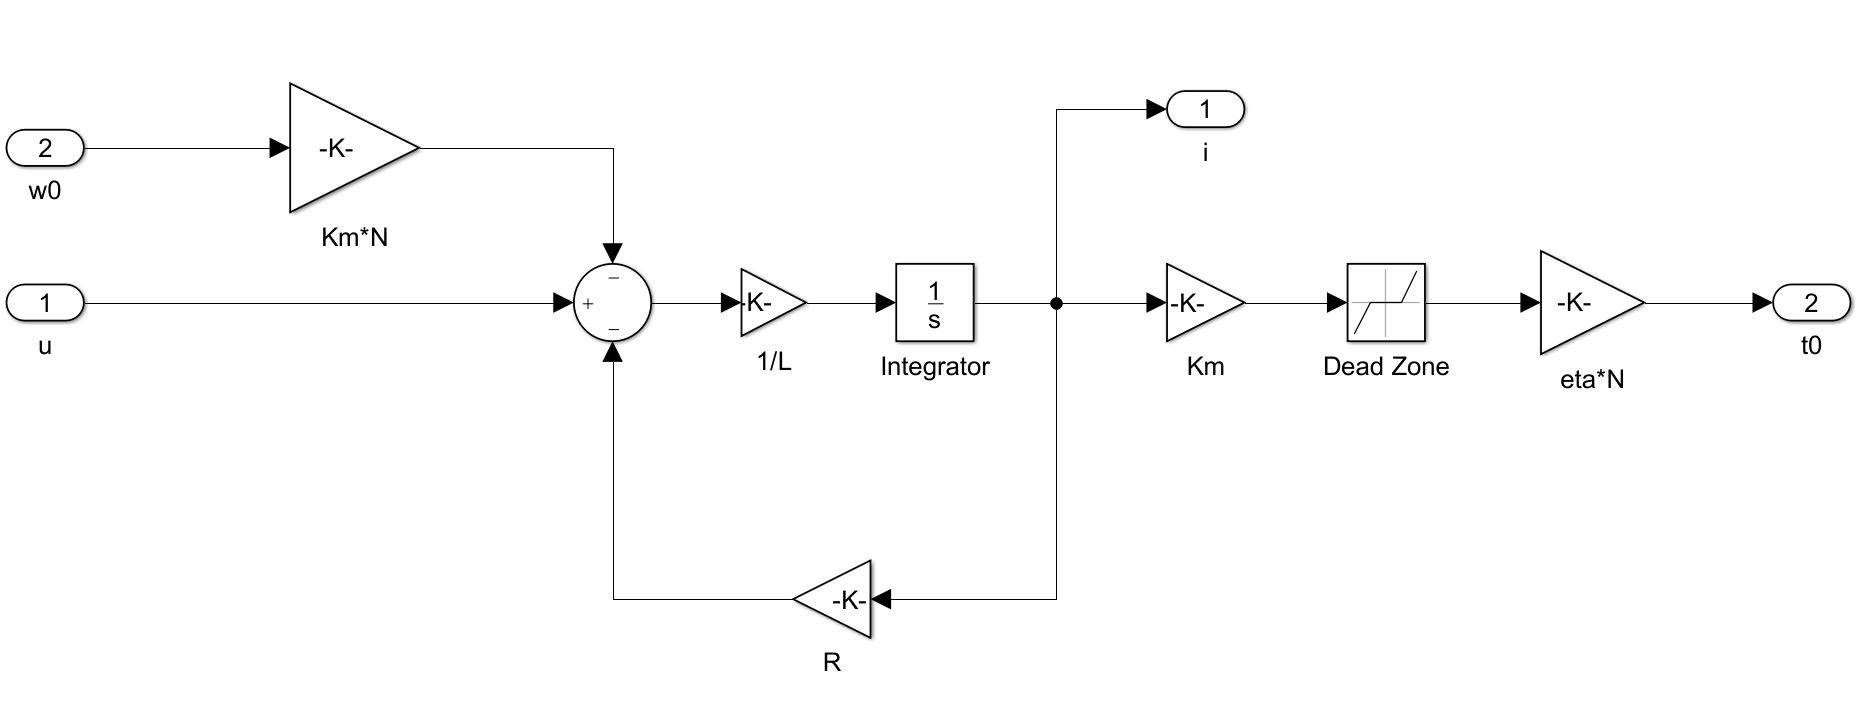
\includegraphics[width=.5\linewidth]{figs/gearbox}
		\caption{Motor Model developed in Assignment 1}
		\label{Motormodel}
	\end{center}
\end{figure}

A control allocation scheme was also developed, which converted the torque desired by the controller into a voltage to be inputted into the motors, based on the equations:
\begin{equation}
\begin{split}
I = \frac{\tau}{\eta NK} + \frac{\tau_{m}}{K} \\
V = RI + \frac{KN\dot{\phi}}{r}
\end{split}
\end{equation}
where $\tau_{m}$ is negative when $\tau<0$   

\newpage
\subsection{Simulink Model}
Thus, the Simulink model shown in Figure \ref{simulink} was developed and used to model the system

\begin{figure}[!h]
	\begin{center}
		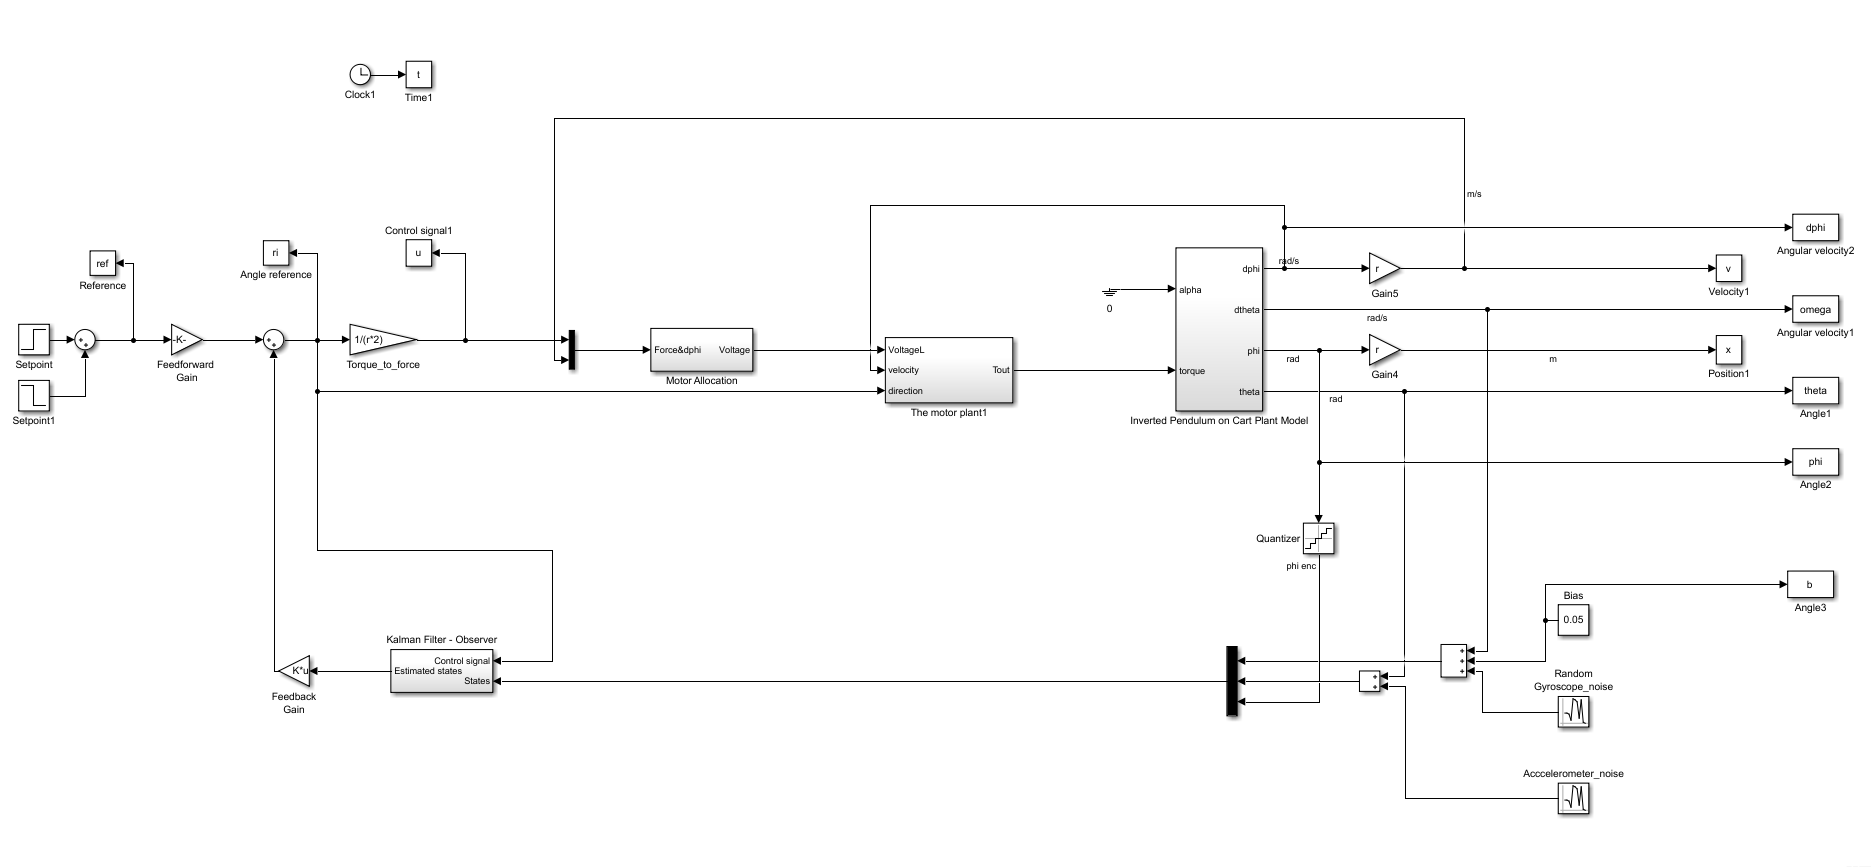
\includegraphics[width=.9\linewidth]{figs/simulink}
		\caption{State feedback Model of the Type II robot with LQR controller and Observer }
		\label{simulink}
	\end{center}
\end{figure}

This model could now be discretized to a control loop rate of $100HZ$ and used to control the type II robot

\newpage
\section{Testing and Commissioning}\label{Testing}
During the assembly process, each subsystem was tested to ensure it functioned as expected.\\ 

\subsection{Electronics} The electrical components were all tested and incrementally soldered to the PCB to validate the circuit. 
\subsection{Model}
The Simulation Model was tested through a variety of inputs, initial angles, inclines and reference signals to ensure robustness. Figure shows the result of simulation in continious time with an intial angle $\theta$ of 5\textsuperscript{o} and step input of 0.1 $rads$

\begin{figure}[!h]
	\begin{center}
		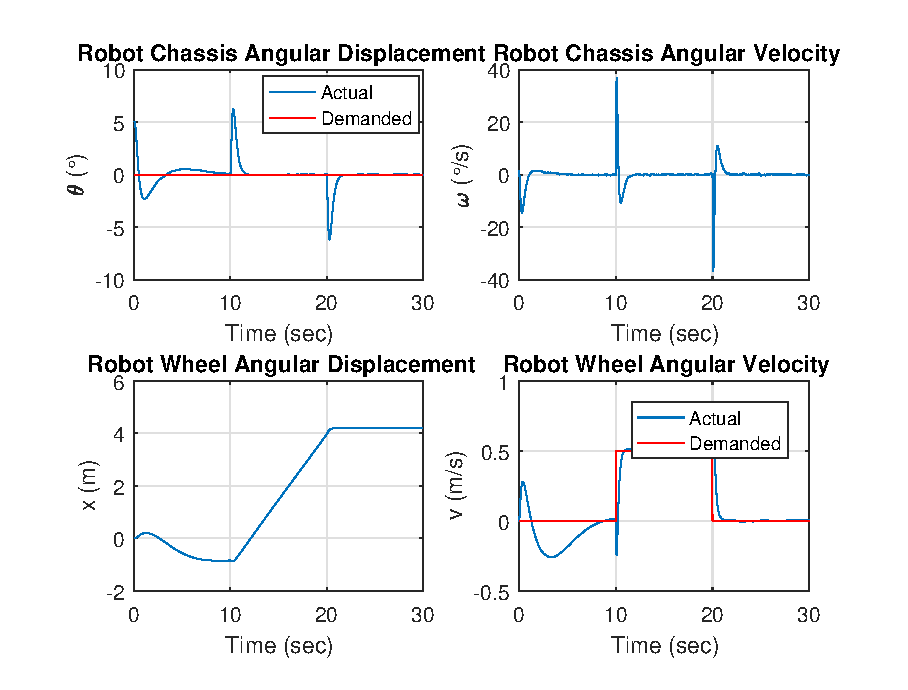
\includegraphics[width=.6\linewidth]{figs/cont1}
		\caption{Model Simulation in Continuous time}
		\label{cont1}
	\end{center}
\end{figure}


\subsection{C code} A string parser, provided during the labs, was used in conjunction with a command table to communicate with the microcontroller. This allowed testing of the motordrivers, encoder, bluetooth module and the translated simulation model functions to ensure that all modules were operating as expected. It also allowed for Hardware-in-the-loop(HIL) testing, during which the micro controller was subjected to simulated real-world inputs and it's response was plotted.




\newpage
\section{Conclusion and Reflection}\label{Conclusion}

After building, testing and commissioning the robot, it was presented on demonstration day where it managed to self stabilize for $\approx$ 5 seconds and would respond to a reference velocity\footnote{Which could not be demonstrated due to its instability}

\subsection{Evaluation}

The project can be evaluated based on the hardware, software, system identification, simulation model and control respectively:


\begin{enumerate}

	\item The model was robust, designed to maximize the available control and kinematic envelope and used optimal power electronics. However, it was quite expensive and parts should have been sourced for much less\footnote{Ordered from China}
	\item The software, especially the Matlab code, is well documented, consistent  and organised. 
	\item The system identification for the motors and chassis are very robust and all of the parameters are automatically exported for use in modeling both in Matlab and in C code. However, the system identification for the Inertia of the wheel and the Motor Driver is lacking
	\item The system is modeled effectively, with sensor quantization and noise as well as actuator limits taken into account 
	\item The system is appropriately controlled using a model based design. However, it lacks anti-windup, advanced estimation\footnote{Sequential Kalman Filtering} and Monte Carlo simulation
\end{enumerate}

\subsection{Reflection}

There were a plethora of mistakes made during the project which hindered its progress. \\ The most significant of these was short-circuiting the PCB and subsequently breaking my components. My PCB design involved a $5V$ and $GND$ plane which i would, through various errors, accidentally connect and short circuit my entire system. As a result, i had to de-solder and re-solder components which wasted approximately 20 hours of my time. As a result, i would suggest testing every solder joint before powering up the circuit. \\

Another major issue was system identification, which i wasted many hours doing incorrectly. For my motors, i took all my initial experimental measurements at at 50\% dutycycle instead of 100\%, which rendered them useless as i learnt that the PWM signal output produced by the motor drivers is non-linear. My initial pendulum swing test was also incorrect, as the motor shaft would lock with the system identification rig and turn the gearbox, causing a great amount of friction that was unaccounted for. I also never managed to compute the Inertia of my motor, which caused my simulation model to be incorrect (which was  tested by incrementing J and noting the significant change it would have on the stability of the system)\\

As a result of all this wasted time, it was also infeasible to implement a better state estimator, such as a sequential Kalman filter. The current estimator was not robust enough for proper estimation, as shown in Appendix \ref{Estimation error}\\

I consider poor system identification, poor state estimation and lack of experience with PCB's to be the primary reasons why my robot balanced as poorly as it did on demonstration day. If I had more time, I would have implemented a Sequential Kalman Filter, done proper system identification to find the inertia of my wheel and on my motor drivers. \\

My overall goal for this project was to have, at the very least, a properly balancing type II robot. Although I fell short on that goal using proper control methods, i did manage to stabilize the robot by intuition\footnote{As seen on the video posted on slack}. I noticed the robot was attempting to stabilize but the control signal was too strong so i factored it down and this resulted in a fairly robust balancing robot. However, i abandoned this method as it didn't help my understanding and treated it as a novelty.

%\subsection{Subsection title}
%You can use subsections within any section of the report. 
%\subsection{Subsection title}
%Recall that you need at least two subsections per section.
%\subsubsection{Subsubsection 1}
%Do not use more than 2 levels of sub-sectioning.
%\subsubsection{Subsubsection 2}
%Do not use more than 2 levels of sub-sectioning.
%
%The rest of the report is organised as follows. Section~\ref{sec:Core Section} describes items related to the core content. Section~\ref{sec:Conclusion} concludes the report. Appendix~\ref{app:Table} shows an example of how to make a Table.
%%%%%%%%%%%%%%%%%%%%%%%%%%%%%%%%
%\section{Core Section}\label{sec:Core Section}
%
%\subsection{Mathematics}
%\LaTeX \ is very good for writing Mathematics. You can write mathematics in the middle of a sentence, like for example $y=m x + h$. Or you can use the \verb|equation| environment as indicated in \eqref{eq:EquationLine} below.
%\begin{equation}\label{eq:EquationLine}
%    y=m x + h.
%\end{equation}
%You can also use equations and tell LaTeX not to number an equation:
%\begin{equation*}
%    z=m_z x^2 + h_z.
%\end{equation*}
%You can use the split command as in \eqref{eq:SS1} below (split gives you only one equation number):
%\begin{equation}\label{eq:SS1}
%    \begin{split}
%        \dot{\mathbf{x}} &= \mathbf{A} \mathbf{x} + \mathbf{B} \mathbf{u}, \\
%        \mathbf{y} &= \mathbf{C} \mathbf{x} + \mathbf{D} \mathbf{u},
%    \end{split}
%\end{equation}
%and you also use numbers for each equation and refer to them separately like in \eqref{eq:State} and \eqref{eq:Output} below:
%\begin{align}
%    \dot{\mathbf{x}} &= \mathbf{A} \mathbf{x} + \mathbf{B} \mathbf{u},  \label{eq:State} \\
%    \mathbf{y} &= \mathbf{C} \mathbf{x} + \mathbf{D} \mathbf{u}. \label{eq:Output} 
%\end{align}
%You can write a matrix like
%\begin{equation*}
%    \mathbf{A} =
%    \begin{bmatrix}
%        A_{11} & A_{12} & \dots & &A_{1n} \\
%        A_{21} & A_{22} &  \dots & &\vdots \\
%        \vdots & \vdots & \ddots& &  \vdots\\
%        A_{m1} & A_{m2} & \dots & &A_{mn}
%    \end{bmatrix}.
%\end{equation*}
%If you want to distinguish vectors from scalars you can use \textbf{bold} for vectors and matrices:
%\begin{equation*} 
%    \begin{split}
%        \dot{\mathbf{x}} &= \mathbf{A} \mathbf{x} + \mathbf{B} u, \\
%        y &= \mathbf{C} \mathbf{x} + \mathbf{D} u,
%    \end{split}
%\end{equation*}
%where $u$ and $y$ are scalar variables and $\mathbf{x}$ is a vector variable.
%You can also write Greek letters in bold: $\boldsymbol{\alpha}$.
%%%%%%%%%%%%%%%%%%%%%%%%%%%
%\subsection{Figures}
%To import the figures from Matlab, follow the following procedure:
%\begin{enumerate}
%    \item Add labels and legends (don't forget to include units in the labels of each axis.)
%    \item From the file menu tag on the figure select export set up
%    \item Change the font size to 14 and click apply to figure
%    \item Export the figure as eps
%    \item Import it in LaTeX using the include graphics within a \verb|figure| environment.
%\end{enumerate}
%%
%\begin{figure}[ht]
%    \begin{center}
%        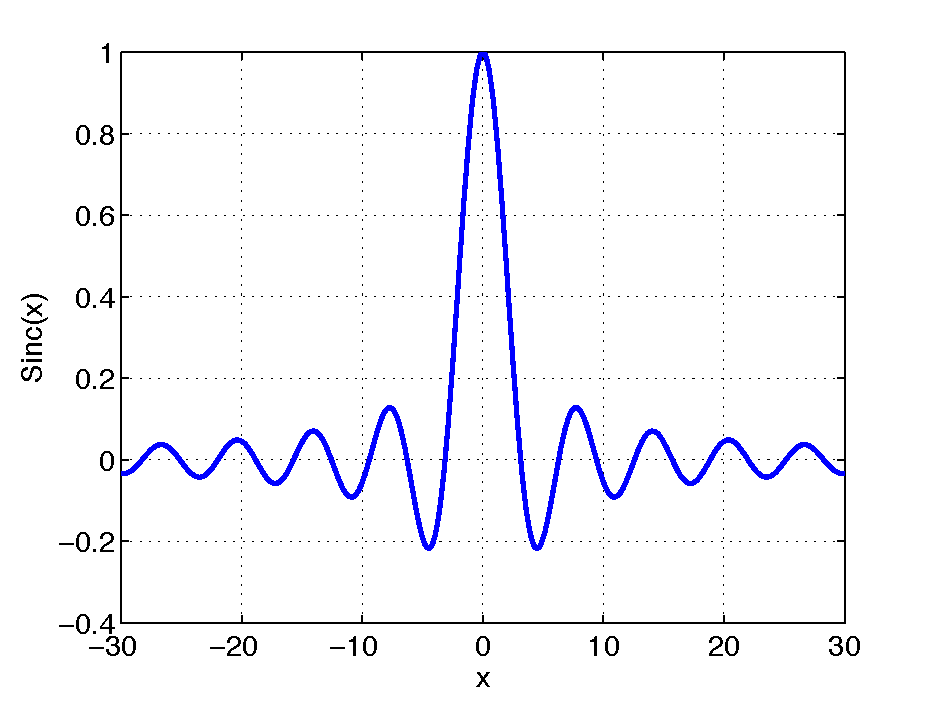
\includegraphics[width=.6\linewidth]{Figures/SincPlot}
%        \caption{Here goes the caption.}
%        \label{fig:Sinc}
%    \end{center}
%\end{figure}
%Figure~\ref{fig:Sinc} shows a shows a plot of the function $\sin(x)/x$. 
%
%If I need to make a simple diagram, I use powerpoint and select the drawing and save it as a pdf. For example, look at Figure~\ref{fig:MechaSys}.
%\begin{figure}[ht]
%    \begin{center}
%        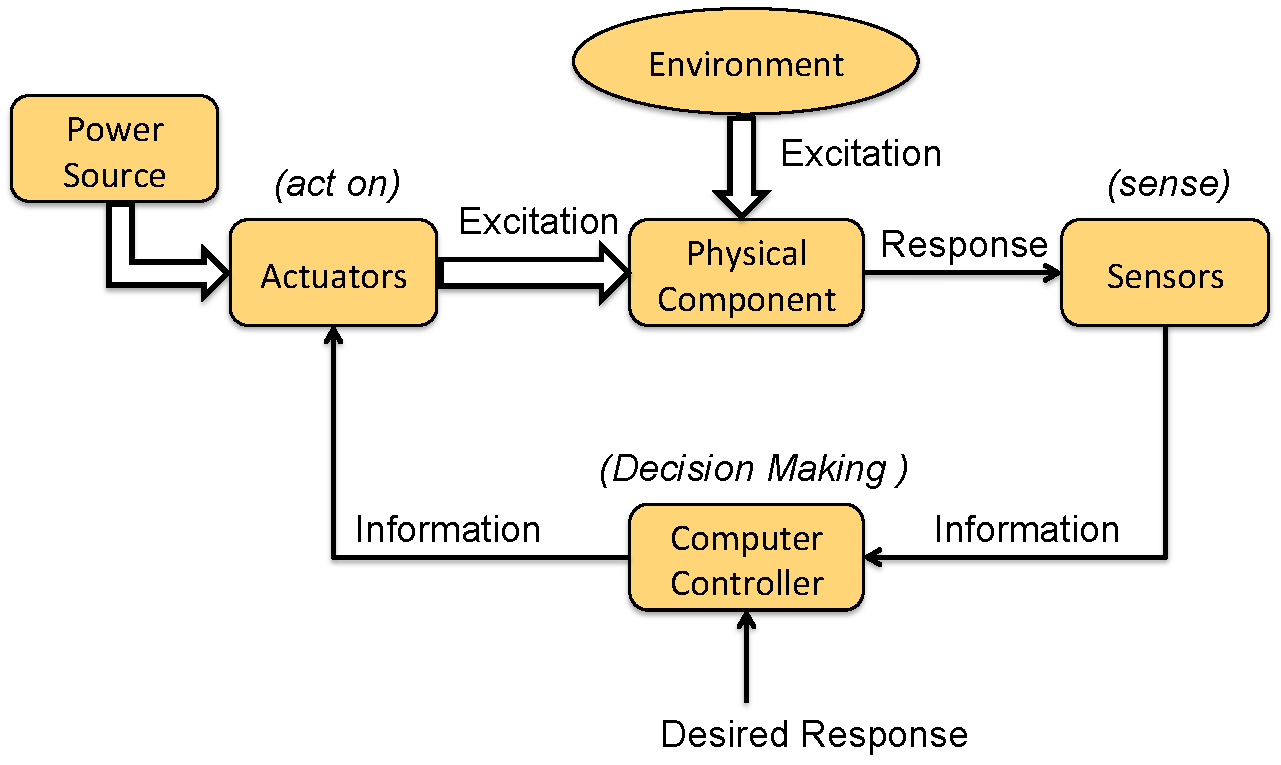
\includegraphics[width=.6\linewidth]{Figures/MechaSys}
%        \caption{Here goes the caption.}
%        \label{fig:MechaSys}
%    \end{center}
%\end{figure}
%%%%%%%%
%\newpage
%\subsection{Lists}
%To create lists use the environments \verb|itemize|, \verb|enumerate|, or \verb|description|
%
%The following is generated using \emph{itemize}
%\begin{itemize}
%    \item This is item 1 
%    \item This is item 2
%\end{itemize}
%%
%The following is generated using \emph{enumerate}
%\begin{enumerate}[1)]
%    \item This is item 1 
%    \begin{enumerate}[a)]
%        \item Subitem a
%        \item Subitem b
%        \begin{enumerate}[i)]
%            \item Subsubitem i
%            \item Subsubitem ii
%        \end{enumerate}
%    \end{enumerate}
%    \item This is item 2
%\end{enumerate}
%%
%The following is generated using \emph{description}
%\begin{description}
%    \item[foo)] This is item 1 
%    \item[bar)] This is item 2
%\end{description}



 %%%%%%%%%%%%%%%%%%%%%%%%%%%%%%%
 \newpage
\section{References and Citations}\label{sec:RefCite}

%%%%%%%%%%%%%%%%%%%%%%%%%%%%%%%%
\bibliographystyle{harvard}
\bibliography{main} % This is the .bib file where the bibliography database is stored

\newpage
\appendix
\section{BOM}\label{BOM}

\begin{table}[!h]
	\centering
	\caption{Bill Of Material for Type II Robot}
	\label{MYBOM}
	\resizebox{\textwidth}{!}{%
		\begin{tabular}{|l|l|l|l|l|}
			\hline
			\textbf{Part}     & \textbf{Name}                                                          & \textbf{Vendor}         & \textbf{Price (exc. Shipping)} & \textbf{Quantity} \\ \hline
			Chassis           &                                                                        & University of Newcastle & \$0.00                         & 1                 \\ \hline
			Motor(s)          & \href{https://www.robotgear.com.au/Product.aspx/Details/4546-19-1-Metal-Gearmotor-37Dx68L-mm-with-64-CPR-Encoder}{19:1 Metal Gearmotor 37Dx68L mm with 64 CPR Encoder}                    & Robot Gear Australia    & \$59.95                        & 2                 \\ \hline
			Motor Driver(s)   & \href{https://core-electronics.com.au/vnh5019-motor-driver-carrier.html}{VNH5019 Motor Driver Carrier}                                           & Core Electronics        & \$32.78                        & 2                 \\ \hline
			Current Sensor(s) & \href{https://core-electronics.com.au/acs711ex-current-sensor-carrier-15-5a-to-15-5a.html}{ACS711EX Current Sensor Carrier -15.5A to +15.5A}                       & Core Electronics        & \$5.57                         & 2                 \\ \hline
			IMU               & \href{https://core-electronics.com.au/mpu-6050-module-3-axis-gyroscope-acce-lerometer.html}{MPU6050}                                                                & Core Electronics        & \$10.95                        & 1                 \\ \hline
			Bluetooth         & \href{https://core-electronics.com.au/bluetooth-module-hc-05.html}{HC-05 Bluetooth Module}                                               & Core Electronics        & \$12.00                        & 1                 \\ \hline
			LCD               & \href{https://core-electronics.com.au/standard-lcd-16x2-extras-white-on-blue.html}{HD44780 LCD 16x2}                                                       & Core Electronics        & \$18.90                        & 1                 \\ \hline
			Switch            & \href{https://www.jaycar.com.au/rocker-switch-illuminated-green-spst-15a-240vac/p/SK0979}{Rocker Switch}                                                          & Jaycar Electronics      & \$3.50                         & 1                 \\ \hline
			Battery           & \href{https://hobbyking.com/en_us/turnigy-5000mah-3s-20c-lipo-pack-xt-90.html?___store=en_us}{Turnigy 5000mAh 3S 20C Lipo Pack w/XT-60}                               & Hobbyking               & \$34.29                        & 1                 \\ \hline
			Charger           & \href{https://tinyurl.com/yd88ryr7}{SkyRC E3 2 - 3Cell 7.4V - 11.1V Lipo Battery Balance Charger}           & Ebay                    & \$26.99                        & 1                 \\ \hline
			Connector         & \href{https://tinyurl.com/y8hshlhf}{XT90 RC Nylon XT-90 Male Female Bullet Connector Plug for Lipo Battery} & Ebay                    & \$6.85                         & 1                 \\ \hline
			Voltage Alarm     & \href{https://tinyurl.com/y7k3g3km}{BX100 1-8S Indicator RC Lipo Battery Tester Low Voltage Buzzer Alarm}   & Ebay                    & \$4.99                         & 1                 \\ \hline
			\textbf{TOTAL}    & \textbf{}                                                              & \textbf{}               & \textbf{\$315.07}              & \textbf{}         \\ \hline
		\end{tabular}%
	}
\end{table}

\section{Inertia of the motor estimation}\label{JsysID}

\begin{figure}[!h]
	\begin{center}
		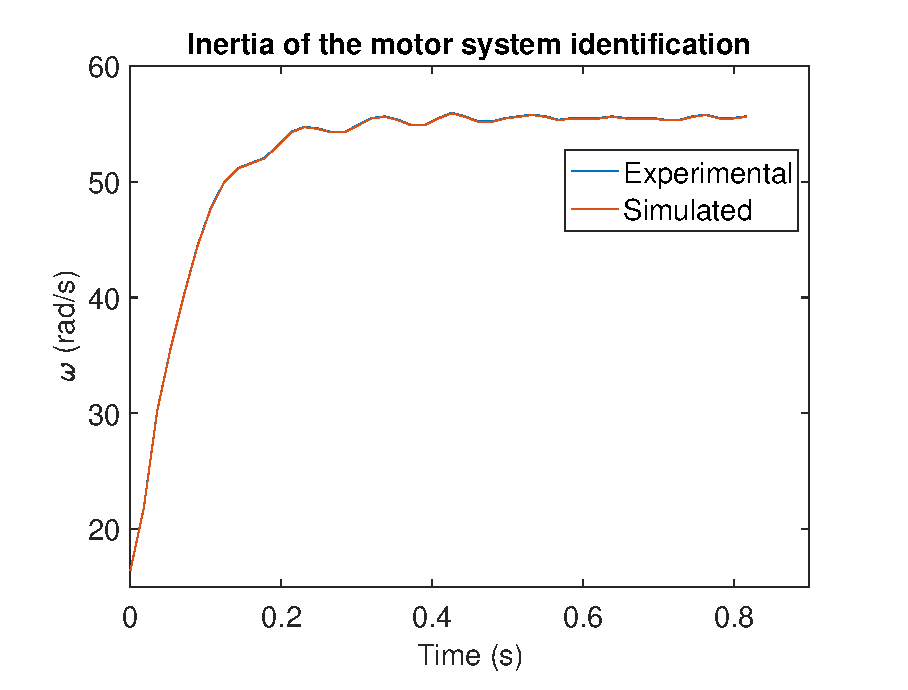
\includegraphics[width=.5\linewidth]{figs/findJ}
		\caption{Angular displacement of the motor shaft over time}
		\label{phi}
	\end{center}
\end{figure}

\newpage
\section{Estimation error}\label{Estimation error}

\begin{figure}[!h]
	\begin{floatrow}
		\ffigbox{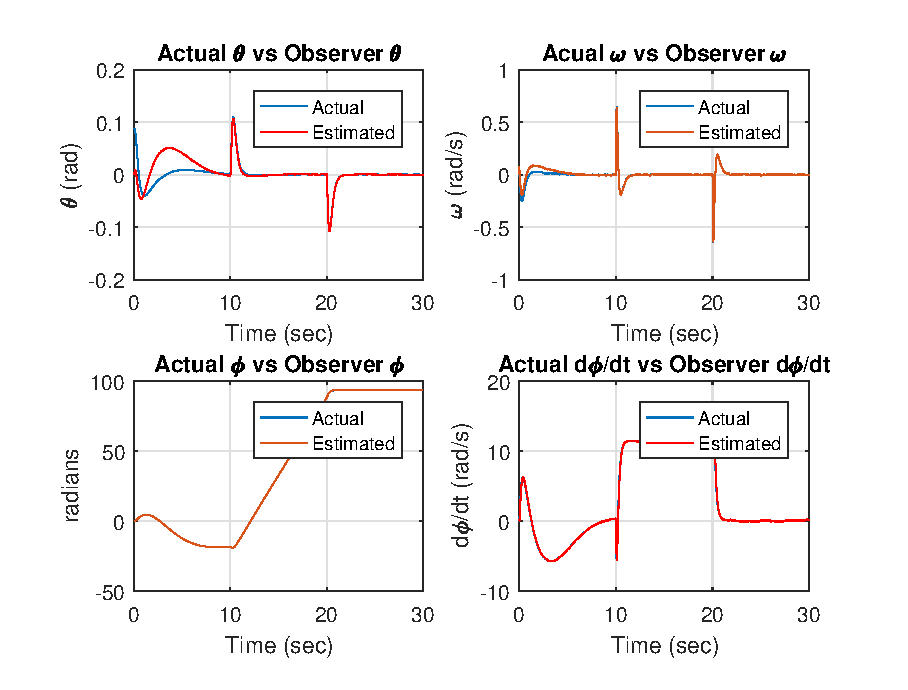
\includegraphics[scale = 0.6]{figs/cont2}}{\caption{Estimated vs Actual states }\label{fiddly}}
		\ffigbox{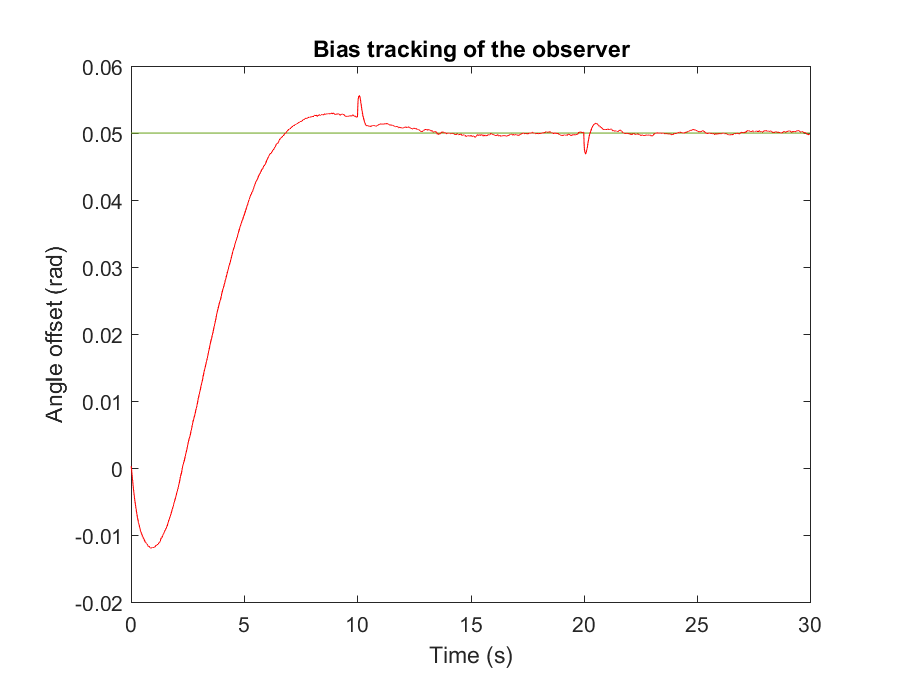
\includegraphics[scale = 0.6]{figs/cont3}}{\caption{Bias estimation }\label{foo}}
	\end{floatrow}
\end{figure}

\end{document}



